En este capitulo que nos conlleva a analizar los actores que ejecutaran la aplicación, los flujos que esta tendrá.

\section{Interacción del Usuario en la Simulación}
\begin{figure}[ht]
\centering
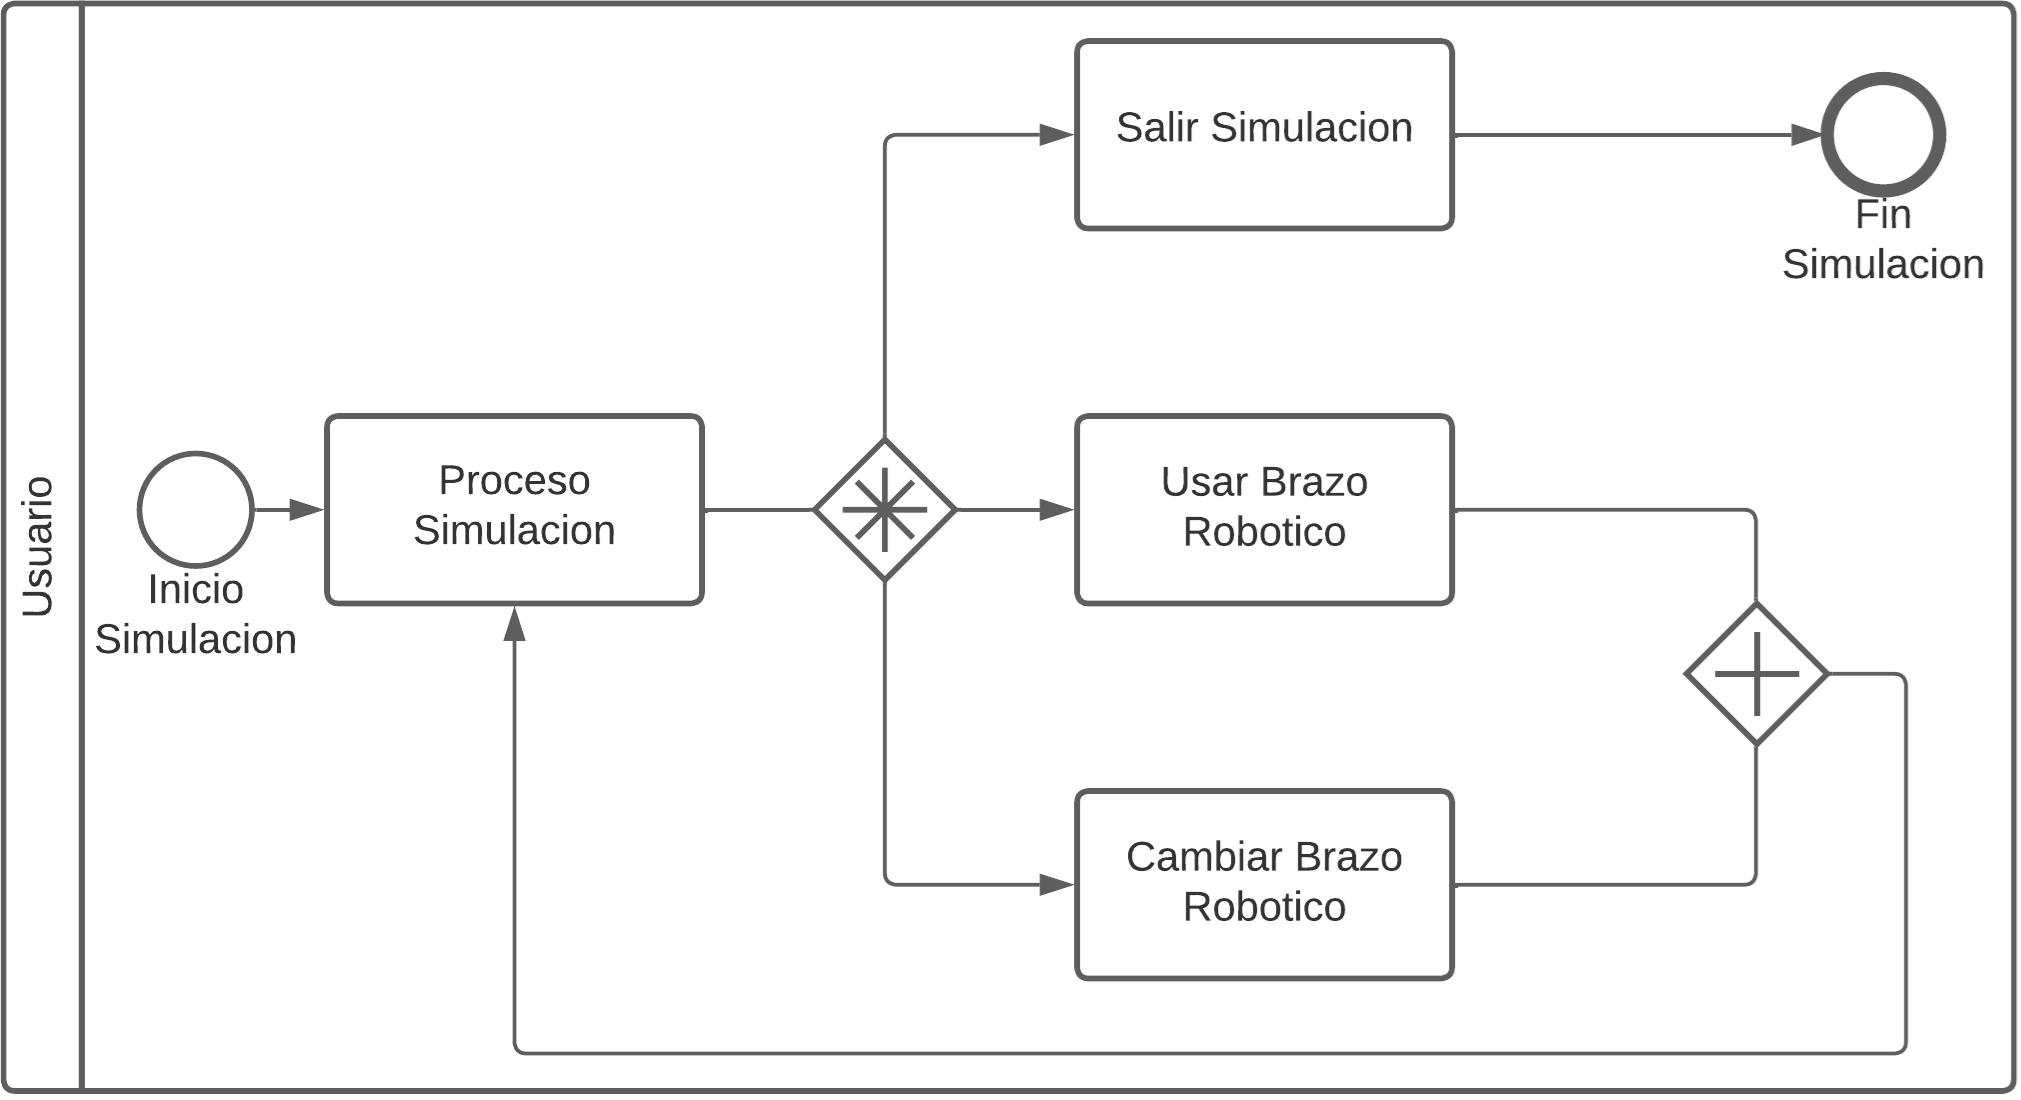
\includegraphics[height=6.83cm]{figures/bpmn.png}
\caption{BPMN de la Interacción}
\label{fig:bpmn}
\end{figure}

En la Figura ~\ref{fig:bpmn} se muestra el proceso de como el usuario interactúa con la simulación, el proceso inicia con el usuario ejecutando la simulación, una vez dentro de esta, el usuario puede elegir entre usar el brazo robótico, cambiar de brazo robótico, con las cuales lo lleva a mantenerse en el proceso de la simulación, por ultimo esta la opción de salir de la simulación que finaliza este proceso

\section{Casos de uso}
\subsection{Actores}
Usuario: Persona que utilizara la aplicación, ya sea estudiante o profesor de la Universidad del Bío-Bío, como también personas externas a esta. El usuario puede utilizar la aplicación completamente.

\subsection{Diagrama de casos de uso y descripción}
Este capítulo destaca los casos de uso del proyecto, ofreciendo una visión rápida de las interacciones que los usuarios pueden realizar.


\textbf{Caso de uso: Uso de Interfaz Principal}
\begin{figure}[ht]
\centering
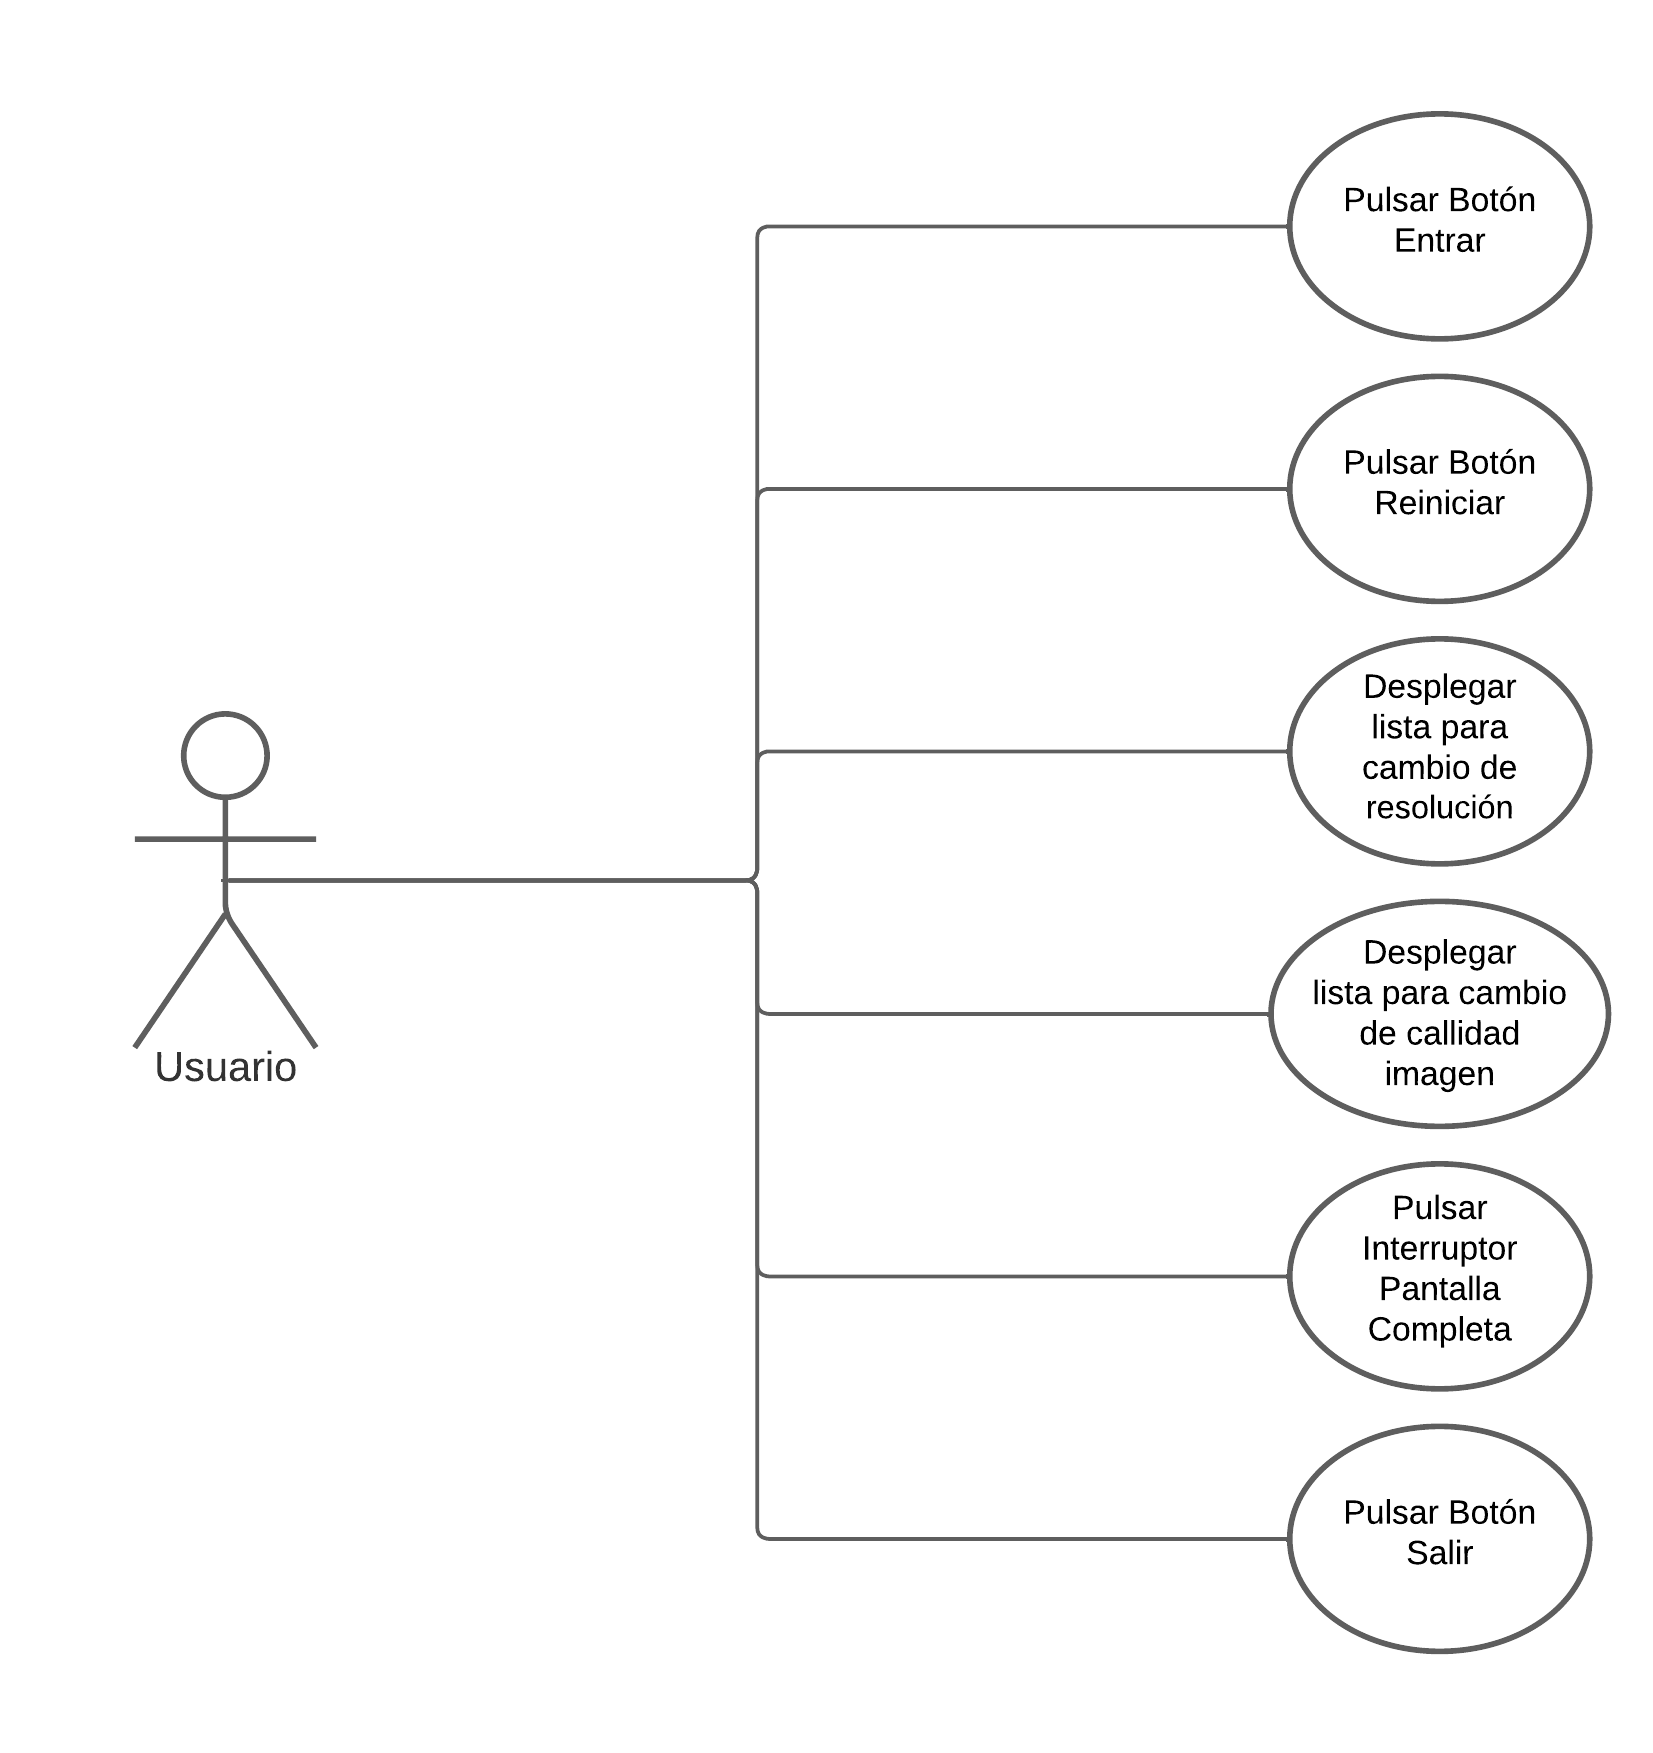
\includegraphics[width=13cm, height=13cm]{figures/cuui.png}
\caption{Diagrama de caso de uso: Usuario}
\label{fig:cuui}
\end{figure}

Como se logra apreciar en la Figura ~\ref{fig:cuui}, se enfoca en la configuración y ajuste de parámetros de la aplicación. Desde reiniciar la simulación hasta cambiar la resolución y calidad de la imagen, estos casos ofrecen opciones para personalizar la configuración de la aplicación según las preferencias del usuario y asi poder abarcar más equipos, por ejemplo, con menos recursos.


\textbf{Caso de uso: Uso de Interfaz dentro de simulación}
\begin{figure}[ht]
\centering
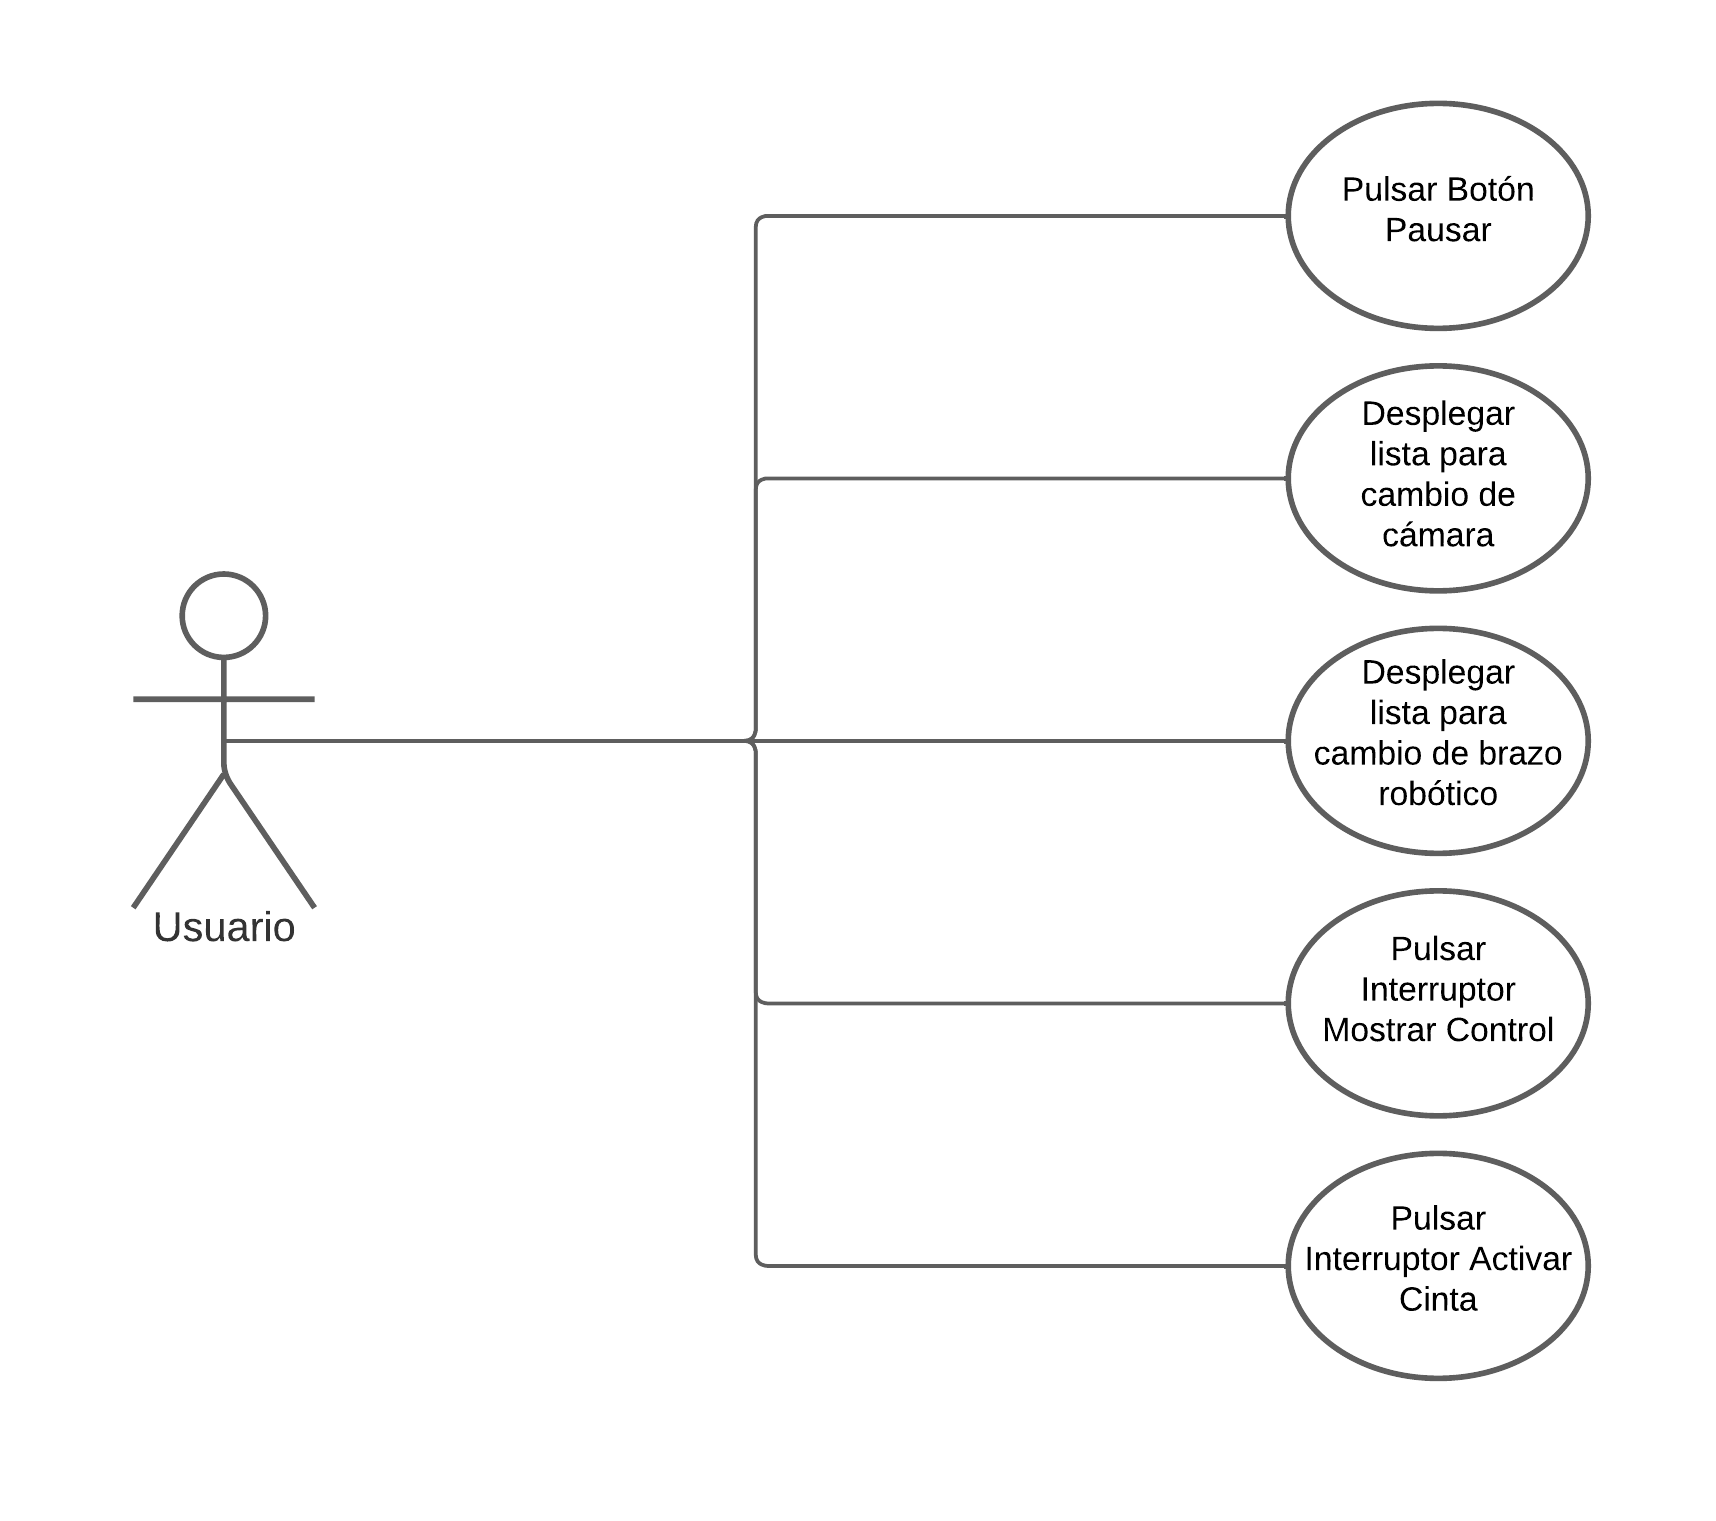
\includegraphics[width=13cm, height=12cm]{figures/cuuisimulacion.png}
\caption{Diagrama de caso de uso: Usuario}
\label{fig:cuuisimulacion}
\end{figure}

Como se logra apreciar en la Figura ~\ref{fig:cuuisimulacion}, esta aborda la navegación y visualización en el sistema. Desde cambiar cámaras hasta activar o desactivar funciones, estos casos permiten a los usuarios personalizar su experiencia de visualización de manera eficiente, cambiar el dispositivo a controlar y cambiar el estado de la cinta transportadora.

\clearpage
\textbf{Caso de uso: Uso de Botonera}
\begin{figure}[ht]
\centering
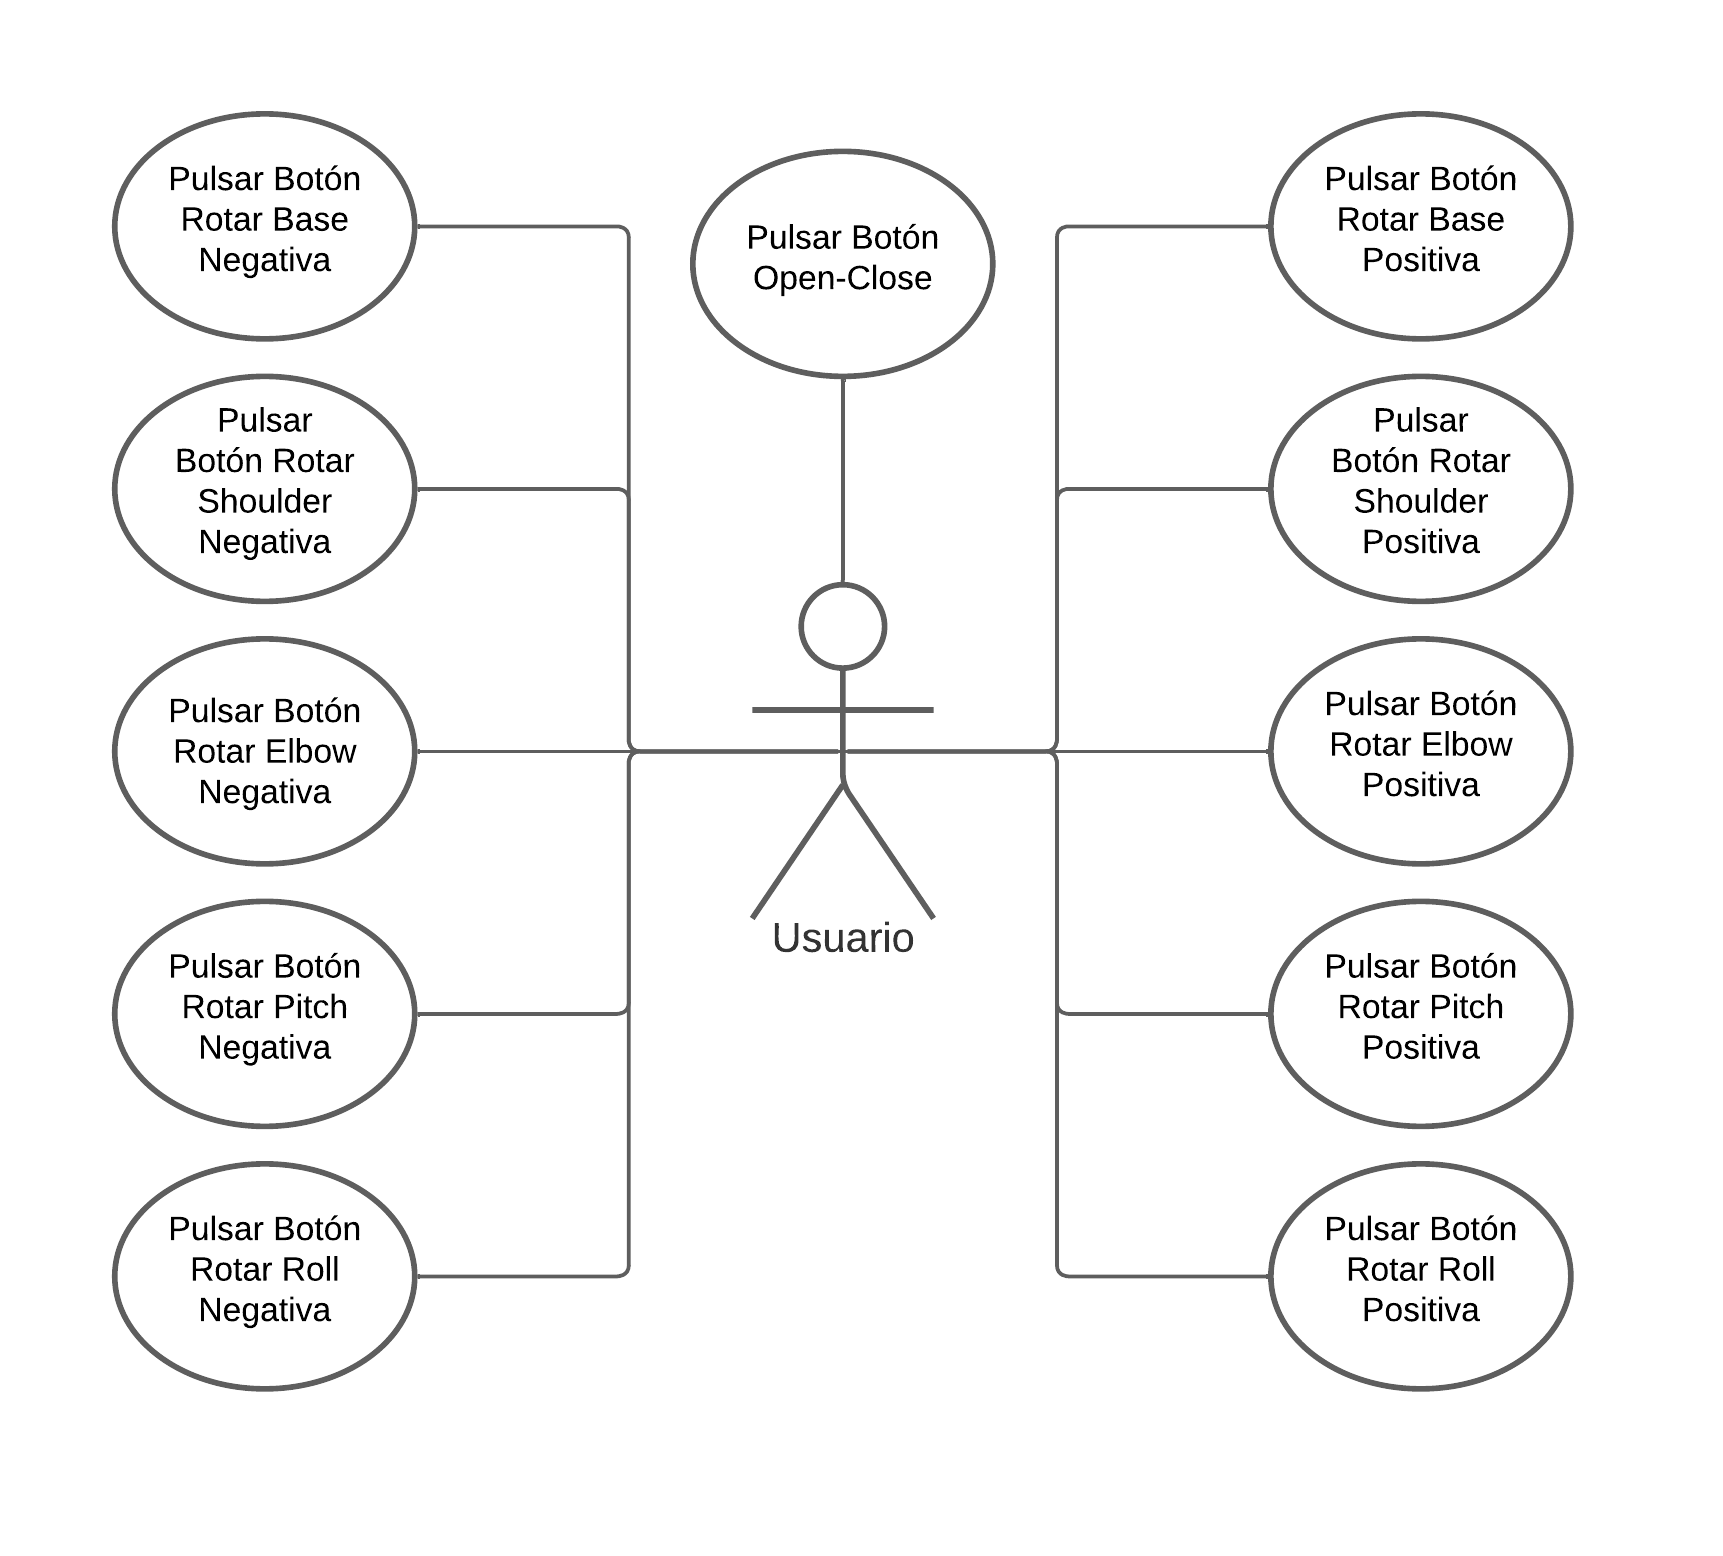
\includegraphics[width=13cm, height=12cm]{figures/cubotonera.png}
\caption{Diagrama de caso de uso: Usuario}
\label{fig:cubotonera}
\end{figure}

Como se logra apreciar en la Figura ~\ref{fig:cubotonera}, se centra en las diversas acciones de movimiento del brazo robot que se encuentran operativas en la botonera. Desde la rotación de articulaciones hasta el control de la pinza, estos casos proporcionan un panorama completo de las capacidades de manipulación del sistema.




\clearpage
\subsection{Especificación de los caso de uso}

\begin{table}[ht!]
\begin{center}
\begin{tabular}{| m{0.19\linewidth} | m{0.75\linewidth} |}
\hline
\multicolumn{2}{ |c| }{Caso de Uso: Pulsar Botón Entrar} \\ \hline
ID & CU-01 \\ \hline
Precondiciones & El actor ejecutó el programa. \\ \hline
Descripción & El actor puede ingresar a la simulación al pulsar el botón correspondiente. \\ \hline
Actores & Usuario \\ \hline
Flujo principal & 

\begin{enumerate}[label=\arabic*.-]
\item El actor visualiza el control de brazo robot.
\item El actor localiza el botón de ''Entrar''.
\item El actor pulsa el botón de ''Entrar''.
\end{enumerate}

\\ \hline
\end{tabular}
\caption{Especificación de casos de uso: Pulsar Botón Entrar}
\end{center}
\end{table}

\begin{table}[ht!]
\begin{center}
\begin{tabular}{| m{0.19\linewidth} | m{0.75\linewidth} |}
\hline
\multicolumn{2}{ |c| }{Caso de Uso: Pulsar Botón Reiniciar} \\ \hline
ID & CU-02 \\ \hline
Precondiciones & El actor ejecutó el programa. \\ \hline
Descripción & El actor puede reiniciar la simulación al pulsar el botón correspondiente. \\ \hline
Actores & Usuario \\ \hline
Flujo principal & 

\begin{enumerate}[label=\arabic*.-]
\item El actor visualiza el control de brazo robot.
\item El actor localiza el botón de ''Reiniciar''.
\item El actor pulsa el botón de ''Reiniciar''.
\end{enumerate}

\\ \hline
\end{tabular}
\caption{Especificación de casos de uso: Pulsar Botón Reiniciar}
\end{center}
\end{table}

\begin{table}[ht!]
\begin{center}
\begin{tabular}{| m{0.19\linewidth} | m{0.75\linewidth} |}
\hline
\multicolumn{2}{ |c| }{Caso de Uso: Desplegar lista para cambio de resolución} \\ \hline
ID & CU-03 \\ \hline
Precondiciones & El actor ejecutó el programa. \\ \hline
Descripción & El actor puede acceder a una lista para cambiar la resolución del sistema al seleccionar la opción correspondiente. \\ \hline
Actores & Usuario \\ \hline
Flujo principal & 

\begin{enumerate}[label=\arabic*.-]
\item El actor visualiza el control de brazo robot.
\item El actor localiza la opción para ''Cambio de Resolución''.
\item El actor despliega la lista para cambio de resolución.
\item El actor cambia la resolución.
\end{enumerate}

\\ \hline
\end{tabular}
\caption{Especificación de casos de uso: Desplegar lista para cambio de resolución}
\end{center}
\end{table}

\begin{table}[ht!]
\begin{center}
\begin{tabular}{| m{0.19\linewidth} | m{0.75\linewidth} |}
\hline
\multicolumn{2}{ |c| }{Caso de Uso: Desplegar lista para cambio de calidad imagen} \\ \hline
ID & CU-04 \\ \hline
Precondiciones & El actor ejecutó el programa. \\ \hline
Descripción & El actor puede acceder a una lista para cambiar la calidad de la imagen del sistema al seleccionar la opción correspondiente. \\ \hline
Actores & Usuario \\ \hline
Flujo principal & 

\begin{enumerate}[label=\arabic*.-]
\item El actor visualiza el control de brazo robot.
\item El actor localiza la opción para ''Cambio de Calidad de Imagen''.
\item El actor despliega la lista para cambio de calidad de imagen.
\end{enumerate}

\\ \hline
\end{tabular}
\caption{Especificación de casos de uso: Desplegar lista para cambio de calidad imagen}
\end{center}
\end{table}

\begin{table}[ht!]
\begin{center}
\begin{tabular}{| m{0.19\linewidth} | m{0.75\linewidth} |}
\hline
\multicolumn{2}{ |c| }{Caso de Uso: Pulsar Interruptor Pantalla Completa} \\ \hline
ID & CU-05 \\ \hline
Precondiciones & El actor ejecutó el programa. \\ \hline
Descripción & El actor puede activar o desactivar el modo de pantalla completa al pulsar el interruptor correspondiente. \\ \hline
Actores & Usuario \\ \hline
Flujo principal & 

\begin{enumerate}[label=\arabic*.-]
\item El actor visualiza el control de brazo robot.
\item El actor localiza el interruptor para ''Pantalla Completa''.
\item El actor pulsa el interruptor para activar o desactivar la pantalla completa.
\end{enumerate}

\\ \hline
\end{tabular}
\caption{Especificación de casos de uso: Pulsar Interruptor Pantalla Completa}
\end{center}
\end{table}

\begin{table}[ht!]
\begin{center}
\begin{tabular}{| m{0.19\linewidth} | m{0.75\linewidth} |}
\hline
\multicolumn{2}{ |c| }{Caso de Uso: Pulsar Botón Salir} \\ \hline
ID & CU-06 \\ \hline
Precondiciones & El actor ejecutó el programa. \\ \hline
Descripción & El actor puede salir del sistema al pulsar el botón correspondiente. \\ \hline
Actores & Usuario \\ \hline
Flujo principal & 

\begin{enumerate}[label=\arabic*.-]
\item El actor visualiza el control de brazo robot.
\item El actor localiza el botón de ''Salir''.
\item El actor pulsa el botón de ''Salir''.
\end{enumerate}

\\ \hline
\end{tabular}
\caption{Especificación de casos de uso: Pulsar Botón Salir}
\end{center}
\end{table}    

\begin{table}[ht!]
\begin{center}
\begin{tabular}{| m{0.19\linewidth} | m{0.75\linewidth} |}
\hline
\multicolumn{2}{ |c| }{Caso de Uso: Pulsar Botón Pausar} \\ \hline
ID & CU-07 \\ \hline
Precondiciones & El actor entró a la simulación. \\ \hline
Descripción & El actor puede pausar la simulación y volver al menu al pulsar el botón correspondiente. \\ \hline
Actores & Usuario \\ \hline
Flujo principal & 

\begin{enumerate}[label=\arabic*.-]
\item El actor visualiza el control de brazo robot.
\item El actor localiza el botón de ''Pausar''.
\item El actor pulsa el botón de ''Pausar''.
\end{enumerate}

\\ \hline
\end{tabular}
\caption{Especificación de casos de uso: Pulsar Botón Pausar}
\end{center}
\end{table}


\begin{table}[ht!]
\begin{center}
\begin{tabular}{| m{0.19\linewidth} | m{0.75\linewidth} |}
\hline
\multicolumn{2}{ |c| }{Caso de Uso: Desplegar lista para cambio de cámara} \\ \hline
ID & CU-08 \\ \hline
Precondiciones & El actor entró a la simulación. \\ \hline
Descripción & El actor puede acceder a una lista para cambiar la cámara del sistema al seleccionar la opción correspondiente. \\ \hline
Actores & Usuario \\ \hline
Flujo principal & 

\begin{enumerate}[label=\arabic*.-]
\item El actor visualiza el control de brazo robot.
\item El actor localiza la opción para ''Cambio de Cámara''.
\item El actor despliega la lista para cambio de cámara.
\item El actor cambia la cámara
\end{enumerate}

\\ \hline
\end{tabular}
\caption{Especificación de casos de uso: Desplegar lista para cambio de cámara}
\end{center}
\end{table}

\begin{table}[ht!]
\begin{center}
\begin{tabular}{| m{0.19\linewidth} | m{0.75\linewidth} |}
\hline
\multicolumn{2}{ |c| }{Caso de Uso: Desplegar lista para cambio de brazo robótico} \\ \hline
ID & CU-09 \\ \hline
Precondiciones & El actor entró a la simulación. \\ \hline
Descripción & El actor puede acceder a una lista para cambiar el brazo robótico al seleccionar la opción correspondiente. \\ \hline
Actores & Usuario \\ \hline
Flujo principal & 

\begin{enumerate}[label=\arabic*.-]
\item El actor visualiza el control de brazo robot.
\item El actor localiza la opción para ''Cambio de Brazo Robótico''.
\item El actor despliega la lista para cambio de brazo robótico.
\item El actor cambia el brazo robótico.
\end{enumerate}

\\ \hline
\end{tabular}
\caption{Especificación de casos de uso: Desplegar lista para cambio de brazo robótico}
\end{center}
\end{table}

\begin{table}[ht!]
\begin{center}
\begin{tabular}{| m{0.19\linewidth} | m{0.75\linewidth} |}
\hline
\multicolumn{2}{ |c| }{Caso de Uso: Pulsar Interruptor Mostrar Control} \\ \hline
ID & CU-10 \\ \hline
Precondiciones & El actor entró a la simulación. \\ \hline
Descripción & El actor puede mostrar u ocultar el control del brazo robot al pulsar el interruptor correspondiente. \\ \hline
Actores & Usuario \\ \hline
Flujo principal & 

\begin{enumerate}[label=\arabic*.-]
\item El actor visualiza el control de brazo robot.
\item El actor localiza el interruptor para ''Mostrar Control''.
\item El actor pulsa el interruptor para mostrar u ocultar el control.
\end{enumerate}

\\ \hline
\end{tabular}
\caption{Especificación de casos de uso: Pulsar Interruptor Mostrar Control}
\end{center}
\end{table}

\begin{table}[ht!]
\begin{center}
\begin{tabular}{| m{0.19\linewidth} | m{0.75\linewidth} |}
\hline
\multicolumn{2}{ |c| }{Caso de Uso: Pulsar Interruptor Activar Cinta} \\ \hline
ID & CU-11 \\ \hline
Precondiciones & El actor entró a la simulación. \\ \hline
Descripción & El actor puede activar o desactivar la cinta del brazo robot al pulsar el interruptor correspondiente. \\ \hline
Actores & Usuario \\ \hline
Flujo principal & 

\begin{enumerate}[label=\arabic*.-]
\item El actor visualiza el control de brazo robot.
\item El actor localiza el interruptor para ''Activar Cinta''.
\item El actor pulsa el interruptor para activar o desactivar la cinta.
\end{enumerate}

\\ \hline
\end{tabular}
\caption{Especificación de casos de uso: Pulsar Interruptor Activar Cinta}
\end{center}
\end{table}

\begin{table}[ht!]
\begin{center}
\begin{tabular}{| m{0.19\linewidth} | m{0.75\linewidth} |}
\hline
\multicolumn{2}{ |c| }{Caso de Uso: Pulsar Botón Rotar Base Negativa} \\ \hline
ID & CU-12 \\ \hline
Precondiciones & El actor entró a la simulación. 

La botonera está visible\\ \hline
Descripción & El actor puede rotar la base del brazo robot en sentido negativo al pulsar el botón correspondiente. \\ \hline
Actores & Usuario \\ \hline
Flujo principal & 

\begin{enumerate}[label=\arabic*.-]
\item El actor visualiza el control de brazo robot.
\item El actor localiza el botón de ''Rotar Base Negativa''.
\item El actor pulsa el botón de ''Rotar Base Negativa''.
\end{enumerate}

\\ \hline
\end{tabular}
\caption{Especificación de casos de uso: Pulsar Botón Rotar Base Negativa}
\end{center}
\end{table}

\begin{table}[ht!]
\begin{center}
\begin{tabular}{| m{0.19\linewidth} | m{0.75\linewidth} |}
\hline
\multicolumn{2}{ |c| }{Caso de Uso: Pulsar Botón Rotar Base Positiva} \\ \hline
ID & CU-13 \\ \hline
Precondiciones & El actor entró a la simulación. 

La botonera está visible\\ \hline
Descripción & El actor puede rotar la base del brazo robot en sentido positivo al pulsar el botón correspondiente. \\ \hline
Actores & Usuario \\ \hline
Flujo principal & 

\begin{enumerate}[label=\arabic*.-]
\item El actor visualiza el control de brazo robot.
\item El actor localiza el botón de ''Rotar Base Positiva''.
\item El actor pulsa el botón de ''Rotar Base Positiva''.
\end{enumerate}

\\ \hline
\end{tabular}
\caption{Especificación de casos de uso: Pulsar Botón Rotar Base Positiva}
\end{center}
\end{table}

\begin{table}[ht!]
\begin{center}
\begin{tabular}{| m{0.19\linewidth} | m{0.75\linewidth} |}
\hline
\multicolumn{2}{ |c| }{Caso de Uso: Pulsar Botón Rotar Shoulder Negativa} \\ \hline
ID & CU-14 \\ \hline
Precondiciones & El actor entró a la simulación. 

La botonera está visible\\ \hline
Descripción & El actor puede rotar la articulación ''Shoulder'' en sentido negativo al pulsar el botón correspondiente. \\ \hline
Actores & Usuario \\ \hline
Flujo principal & 

\begin{enumerate}[label=\arabic*.-]
\item El actor visualiza el control de brazo robot.
\item El actor localiza el botón de ''Rotar Shoulder Negativa''.
\item El actor pulsa el botón de ''Rotar Shoulder Negativa''.
\end{enumerate}

\\ \hline
\end{tabular}
\caption{Especificación de casos de uso: Pulsar Botón Rotar Shoulder Negativa}
\end{center}
\end{table}

\begin{table}[ht!]
\begin{center}
\begin{tabular}{| m{0.19\linewidth} | m{0.75\linewidth} |}
\hline
\multicolumn{2}{ |c| }{Caso de Uso: Pulsar Botón Rotar Shoulder Positiva} \\ \hline
ID & CU-15 \\ \hline
Precondiciones & El actor entró a la simulación. 

La botonera está visible\\ \hline
Descripción & El actor puede rotar la articulación ''Shoulder'' en sentido positivo al pulsar el botón correspondiente. \\ \hline
Actores & Usuario \\ \hline
Flujo principal & 

\begin{enumerate}[label=\arabic*.-]
\item El actor visualiza el control de brazo robot.
\item El actor localiza el botón de ''Rotar Shoulder Positiva''.
\item El actor pulsa el botón de ''Rotar Shoulder Positiva''.
\end{enumerate}

\\ \hline
\end{tabular}
\caption{Especificación de casos de uso: Pulsar Botón Rotar Shoulder Positiva}
\end{center}
\end{table}

\begin{table}[ht!]
\begin{center}
\begin{tabular}{| m{0.19\linewidth} | m{0.75\linewidth} |}
\hline
\multicolumn{2}{ |c| }{Caso de Uso: Pulsar Botón Open-Close} \\ \hline
ID & CU-16 \\ \hline
Precondiciones & El actor entró a la simulación. 

La botonera está visible\\ \hline
Descripción & El actor puede abrir o cerrar la pinza del brazo robot al pulsar el botón correspondiente. \\ \hline
Actores & Usuario \\ \hline
Flujo principal & 

\begin{enumerate}[label=\arabic*.-]
\item El actor visualiza el control de brazo robot.
\item El actor localiza el botón ''Open-Close''.
\item El actor pulsa el botón para abrir o cerrar la pinza.
\end{enumerate}

\\ \hline
\end{tabular}
\caption{Especificación de casos de uso: Pulsar Botón Open-Close}
\end{center}
\end{table}

\begin{table}[ht!]
\begin{center}
\begin{tabular}{| m{0.19\linewidth} | m{0.75\linewidth} |}
\hline
\multicolumn{2}{ |c| }{Caso de Uso: Pulsar Botón Rotar Elbow Negativa} \\ \hline
ID & CU-17 \\ \hline
Precondiciones & El actor entró a la simulación. 

La botonera está visible\\ \hline
Descripción & El actor puede rotar la articulación ''Elbow'' en sentido negativo al pulsar el botón correspondiente. \\ \hline
Actores & Usuario \\ \hline
Flujo principal & 

\begin{enumerate}[label=\arabic*.-]
\item El actor visualiza el control de brazo robot.
\item El actor localiza el botón de ''Rotar Elbow Negativa''.
\item El actor pulsa el botón de ''Rotar Elbow Negativa''.
\end{enumerate}

\\ \hline
\end{tabular}
\caption{Especificación de casos de uso: Pulsar Botón Rotar Elbow Negativa}
\end{center}
\end{table}

\begin{table}[ht!]
\begin{center}
\begin{tabular}{| m{0.19\linewidth} | m{0.75\linewidth} |}
\hline
\multicolumn{2}{ |c| }{Caso de Uso: Pulsar Botón Rotar Elbow Positiva} \\ \hline
ID & CU-18 \\ \hline
Precondiciones & El actor entró a la simulación. 

La botonera está visible\\ \hline
Descripción & El actor puede rotar la articulación ''Elbow'' en sentido positivo al pulsar el botón correspondiente. \\ \hline
Actores & Usuario \\ \hline
Flujo principal & 

\begin{enumerate}[label=\arabic*.-]
\item El actor visualiza el control de brazo robot.
\item El actor localiza el botón de ''Rotar Elbow Positiva''.
\item El actor pulsa el botón de ''Rotar Elbow Positiva''.
\end{enumerate}

\\ \hline
\end{tabular}
\caption{Especificación de casos de uso: Pulsar Botón Rotar Elbow Positiva}
\end{center}
\end{table}

\begin{table}[ht!]
\begin{center}
\begin{tabular}{| m{0.19\linewidth} | m{0.75\linewidth} |}
\hline
\multicolumn{2}{ |c| }{Caso de Uso: Pulsar Botón Rotar Pitch Negativa} \\ \hline
ID & CU-19 \\ \hline
Precondiciones & El actor entró a la simulación. 

La botonera está visible\\ \hline
Descripción & El actor puede rotar la articulación ''Pitch'' en sentido negativo al pulsar el botón correspondiente. \\ \hline
Actores & Usuario \\ \hline
Flujo principal & 

\begin{enumerate}[label=\arabic*.-]
\item El actor visualiza el control de brazo robot.
\item El actor localiza el botón de ''Rotar Pitch Negativa''.
\item El actor pulsa el botón de ''Rotar Pitch Negativa''.
\end{enumerate}

\\ \hline
\end{tabular}
\caption{Especificación de casos de uso: Pulsar Botón Rotar Pitch Negativa}
\end{center}
\end{table}

\begin{table}[ht!]
\begin{center}
\begin{tabular}{| m{0.19\linewidth} | m{0.75\linewidth} |}
\hline
\multicolumn{2}{ |c| }{Caso de Uso: Pulsar Botón Rotar Pitch Positiva} \\ \hline
ID & CU-20 \\ \hline
Precondiciones & El actor entró a la simulación. 

La botonera está visible\\ \hline
Descripción & El actor puede rotar la articulación ''Pitch'' en sentido positivo al pulsar el botón correspondiente. \\ \hline
Actores & Usuario \\ \hline
Flujo principal & 

\begin{enumerate}[label=\arabic*.-]
\item El actor visualiza el control de brazo robot.
\item El actor localiza el botón de ''Rotar Pitch Positiva''.
\item El actor pulsa el botón de ''Rotar Pitch Positiva''.
\end{enumerate}

\\ \hline
\end{tabular}
\caption{Especificación de casos de uso: Pulsar Botón Rotar Pitch Positiva}
\end{center}
\end{table}

\begin{table}[ht!]
\begin{center}
\begin{tabular}{| m{0.19\linewidth} | m{0.75\linewidth} |}
\hline
\multicolumn{2}{ |c| }{Caso de Uso: Pulsar Botón Rotar Roll Negativa} \\ \hline
ID & CU-21 \\ \hline
Precondiciones & El actor entró a la simulación. 

La botonera está visible\\ \hline
Descripción & El actor puede rotar la articulación ''Roll'' en sentido negativo al pulsar el botón correspondiente. \\ \hline
Actores & Usuario \\ \hline
Flujo principal & 

\begin{enumerate}[label=\arabic*.-]
\item El actor visualiza el control de brazo robot.
\item El actor localiza el botón de ''Rotar Roll Negativa''.
\item El actor pulsa el botón de ''Rotar Roll Negativa''.
\end{enumerate}

\\ \hline
\end{tabular}
\caption{Especificación de casos de uso: Pulsar Botón Rotar Roll Negativa}
\end{center}
\end{table}

\begin{table}[ht!]
\begin{center}
\begin{tabular}{| m{0.19\linewidth} | m{0.75\linewidth} |}
\hline
\multicolumn{2}{ |c| }{Caso de Uso: Pulsar Botón Rotar Roll Positiva} \\ \hline
ID & CU-22 \\ \hline
Precondiciones & El actor entró a la simulación. 

La botonera está visible\\ \hline
Descripción & El actor puede rotar la articulación ''Roll'' en sentido positivo al pulsar el botón correspondiente. \\ \hline
Actores & Usuario \\ \hline
Flujo principal & 

\begin{enumerate}[label=\arabic*.-]
\item El actor visualiza el control de brazo robot.
\item El actor localiza el botón de ''Rotar Roll Positiva''.
\item El actor pulsa el botón de ''Rotar Roll Positiva''.
\end{enumerate}

\\ \hline
\end{tabular}
\caption{Especificación de casos de uso: Pulsar Botón Rotar Roll Positiva}
\end{center}
\end{table}
